% Template pour faire aide-mémoire
\documentclass[10pt, french]{article}\usepackage[]{graphicx}\usepackage[]{color}
% maxwidth is the original width if it is less than linewidth
% otherwise use linewidth (to make sure the graphics do not exceed the margin)
\makeatletter
\def\maxwidth{ %
  \ifdim\Gin@nat@width>\linewidth
    \linewidth
  \else
    \Gin@nat@width
  \fi
}
\makeatother

\definecolor{fgcolor}{rgb}{0.345, 0.345, 0.345}
\newcommand{\hlnum}[1]{\textcolor[rgb]{0.686,0.059,0.569}{#1}}%
\newcommand{\hlstr}[1]{\textcolor[rgb]{0.192,0.494,0.8}{#1}}%
\newcommand{\hlcom}[1]{\textcolor[rgb]{0.678,0.584,0.686}{\textit{#1}}}%
\newcommand{\hlopt}[1]{\textcolor[rgb]{0,0,0}{#1}}%
\newcommand{\hlstd}[1]{\textcolor[rgb]{0.345,0.345,0.345}{#1}}%
\newcommand{\hlkwa}[1]{\textcolor[rgb]{0.161,0.373,0.58}{\textbf{#1}}}%
\newcommand{\hlkwb}[1]{\textcolor[rgb]{0.69,0.353,0.396}{#1}}%
\newcommand{\hlkwc}[1]{\textcolor[rgb]{0.333,0.667,0.333}{#1}}%
\newcommand{\hlkwd}[1]{\textcolor[rgb]{0.737,0.353,0.396}{\textbf{#1}}}%
\let\hlipl\hlkwb

\usepackage{framed}
\makeatletter
\newenvironment{kframe}{%
 \def\at@end@of@kframe{}%
 \ifinner\ifhmode%
  \def\at@end@of@kframe{\end{minipage}}%
  \begin{minipage}{\columnwidth}%
 \fi\fi%
 \def\FrameCommand##1{\hskip\@totalleftmargin \hskip-\fboxsep
 \colorbox{shadecolor}{##1}\hskip-\fboxsep
     % There is no \\@totalrightmargin, so:
     \hskip-\linewidth \hskip-\@totalleftmargin \hskip\columnwidth}%
 \MakeFramed {\advance\hsize-\width
   \@totalleftmargin\z@ \linewidth\hsize
   \@setminipage}}%
 {\par\unskip\endMakeFramed%
 \at@end@of@kframe}
\makeatother

\definecolor{shadecolor}{rgb}{.97, .97, .97}
\definecolor{messagecolor}{rgb}{0, 0, 0}
\definecolor{warningcolor}{rgb}{1, 0, 1}
\definecolor{errorcolor}{rgb}{1, 0, 0}
\newenvironment{knitrout}{}{} % an empty environment to be redefined in TeX

\usepackage{alltt}

%% -----------------------------
%% Préambule
%% -----------------------------
\input{../../cheatsht-preamble-general.tex}
%% -----------------------------
%% Variable definition
%% -----------------------------
\def\cours{MAS-I}
\def\sigle{(CAS)}
%
% 	Save more space than default
%
\setlength{\abovedisplayskip}{-15pt}
\setlist{leftmargin=*}
\setcounter{secnumdepth}{0}
%
%	Extra math symbols
%
\usepackage{mathrsfs}

%% -----------------------------
%% 	Colour setup for sections
%% -----------------------------
\def\SectionColor{cobalt}
\def\SubSectionColor{azure(colorwheel)}
\def\SubSubSectionColor{azure(colorwheel)}
%% -----------------------------

%% -----------------------------
%% Color definitions
%% -----------------------------
\definecolor{indigo(web)}{rgb}{0.29, 0.0, 0.51}
\definecolor{cobalt}{rgb}{0.0, 0.28, 0.67}
\definecolor{azure(colorwheel)}{rgb}{0.0, 0.5, 1.0}
%% -----------------------------
%% Variable definition
%% -----------------------------
%%
%% Matrix notation variable (bold style)
%%
\newcommand\cololine[2]{\colorlet{temp}{.}\color{#1}\bar{\color{temp}#2}\color{temp}}
\newcommand\colbar[2]{\colorlet{temp}{.}\color{#1}\bar{\color{temp}#2}\color{temp}}
\usepackage{scalerel,stackengine,amsmath}

%%%	------------------------
%%%	NOTES
%%%	+	R setup
%%%	------------------------
\usetikzlibrary{fit, matrix}
\definecolor{ballblue}{rgb}{0.13, 0.67, 0.8}
\definecolor{darkgreen}{rgb}{0.0, 0.2, 0.13}
\definecolor{rstudioblue}{RGB}{247, 247, 247}
\lstset{language=R,
    basicstyle=\small\ttfamily,
    stringstyle=\color{darkgreen},
    otherkeywords={0,1,2,3,4,5,6,7,8,9},
    morekeywords={TRUE,FALSE},
    deletekeywords={data,frame,length,as,character},
    keywordstyle=\color{blue},
    commentstyle=\color{darkgreen},
}


\IfFileExists{upquote.sty}{\usepackage{upquote}}{}
\begin{document}

\part{\texttt{R} functions}
\section{Time Series}
\subsection{Time Series Data (Introductory Time Series with \texttt{R})}

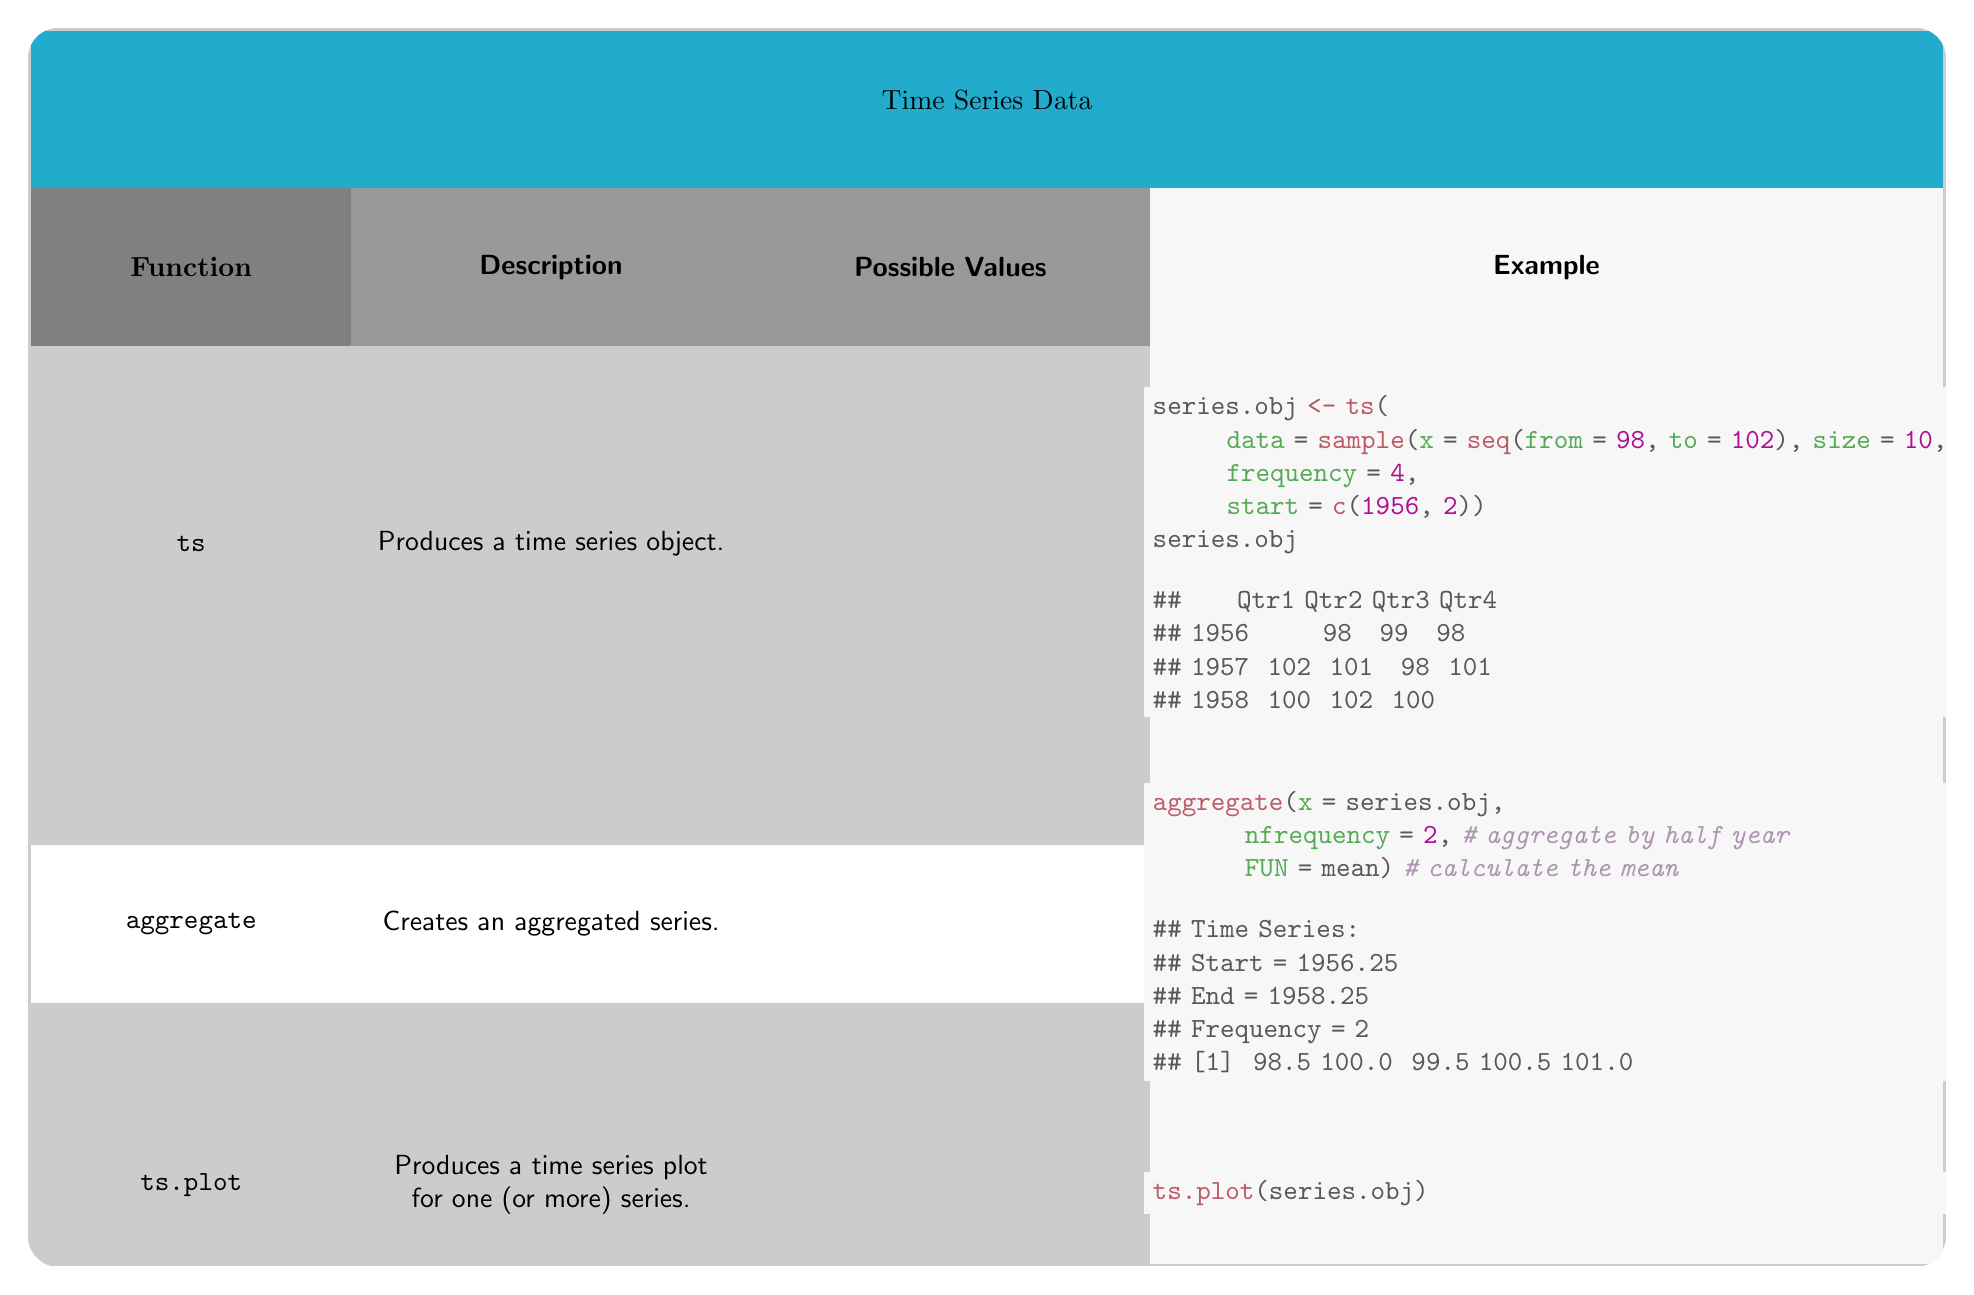
\begin{tikzpicture}
\clip node (m) [
	matrix,
	matrix of nodes,
	fill = black!20, % alternating rows color
	inner sep = 1pt, % width of exterior line
	nodes in empty cells,
	nodes = {
		minimum height = 2cm,
		minimum width = 2.6cm,
		anchor = center,
		outer sep = 1pt,
		font = \sffamily
	},
	row 1/.style = {
		nodes = {
			fill = ballblue,  % header colour
			text = white,
			font = \bfseries
		}
	},
	column 1/.style = {
		text width = 4cm, 
		align = center,
		nodes = {
			font = \bfseries
		},
		every even row/.style = {
			nodes = {
				fill = white
			}
		}
	},
	column 2/.style = {
		text width = 5cm,
		align = center,
		every even row/.style = {nodes = {fill = white}},
	},
	column 3/.style = {
		text width = 5cm,
		align = center,
		every even row/.style = {nodes = {fill = white}},
	},
	column 4/.style = {
		text width = 10cm,
		align = center,
		nodes = {fill = rstudioblue}
	},
	row 2 column 1/.style = {nodes = {fill = gray}},
	prefix after command = {
		[rounded corners = 4mm] (m.north east) rectangle (m.south west)
	},
	row 2 column 2/.style = {nodes = {fill = gray!80!white}},
	prefix after command = {
		[rounded corners = 4mm] (m.north east) rectangle (m.south west)
	},
	row 2 column 3/.style = {nodes = {fill = gray!80!white}},
	prefix after command = {
		[rounded corners = 4mm] (m.north east) rectangle (m.south west)
	}
] {
			&			&			&			\\
	\textbf{Function}	&	\textbf{Description}	&	\textbf{Possible Values}	&	\textbf{Example} \\
	\texttt{ts}		&	Produces a time series object.	&		&	
\begin{knitrout}
\definecolor{shadecolor}{rgb}{0.969, 0.969, 0.969}\color{fgcolor}\begin{kframe}
\begin{alltt}
\hlstd{series.obj} \hlkwb{<-} \hlkwd{ts}\hlstd{(}
        \hlkwc{data} \hlstd{=} \hlkwd{sample}\hlstd{(}\hlkwc{x} \hlstd{=} \hlkwd{seq}\hlstd{(}\hlkwc{from} \hlstd{=} \hlnum{98}\hlstd{,} \hlkwc{to} \hlstd{=} \hlnum{102}\hlstd{),} \hlkwc{size} \hlstd{=} \hlnum{10}\hlstd{,} \hlkwc{replace} \hlstd{= T),}
        \hlkwc{frequency} \hlstd{=} \hlnum{4}\hlstd{,}
        \hlkwc{start} \hlstd{=} \hlkwd{c}\hlstd{(}\hlnum{1956}\hlstd{,} \hlnum{2}\hlstd{))}
\hlstd{series.obj}
\end{alltt}
\begin{verbatim}
##      Qtr1 Qtr2 Qtr3 Qtr4
## 1956        98   99   98
## 1957  102  101   98  101
## 1958  100  102  100
\end{verbatim}
\end{kframe}
\end{knitrout}
   	\\
	\texttt{aggregate}		&	Creates an aggregated series.	&		&	
\begin{knitrout}
\definecolor{shadecolor}{rgb}{0.969, 0.969, 0.969}\color{fgcolor}\begin{kframe}
\begin{alltt}
\hlkwd{aggregate}\hlstd{(}\hlkwc{x} \hlstd{= series.obj,}
          \hlkwc{nfrequency} \hlstd{=} \hlnum{2}\hlstd{,} \hlcom{# aggregate by half year}
          \hlkwc{FUN} \hlstd{= mean)} \hlcom{# calculate the mean}
\end{alltt}
\begin{verbatim}
## Time Series:
## Start = 1956.25 
## End = 1958.25 
## Frequency = 2 
## [1]  98.5 100.0  99.5 100.5 101.0
\end{verbatim}
\end{kframe}
\end{knitrout}
	\\
	\texttt{ts.plot}		&	Produces a time series plot for one (or more) series.	&	 	&	
\begin{knitrout}
\definecolor{shadecolor}{rgb}{0.969, 0.969, 0.969}\color{fgcolor}\begin{kframe}
\begin{alltt}
\hlkwd{ts.plot}\hlstd{(series.obj)}
\end{alltt}
\end{kframe}
\end{knitrout}
	\\
};
    \node[fit=(m-1-1)(m-1-4)]{Time Series Data};
\end{tikzpicture}

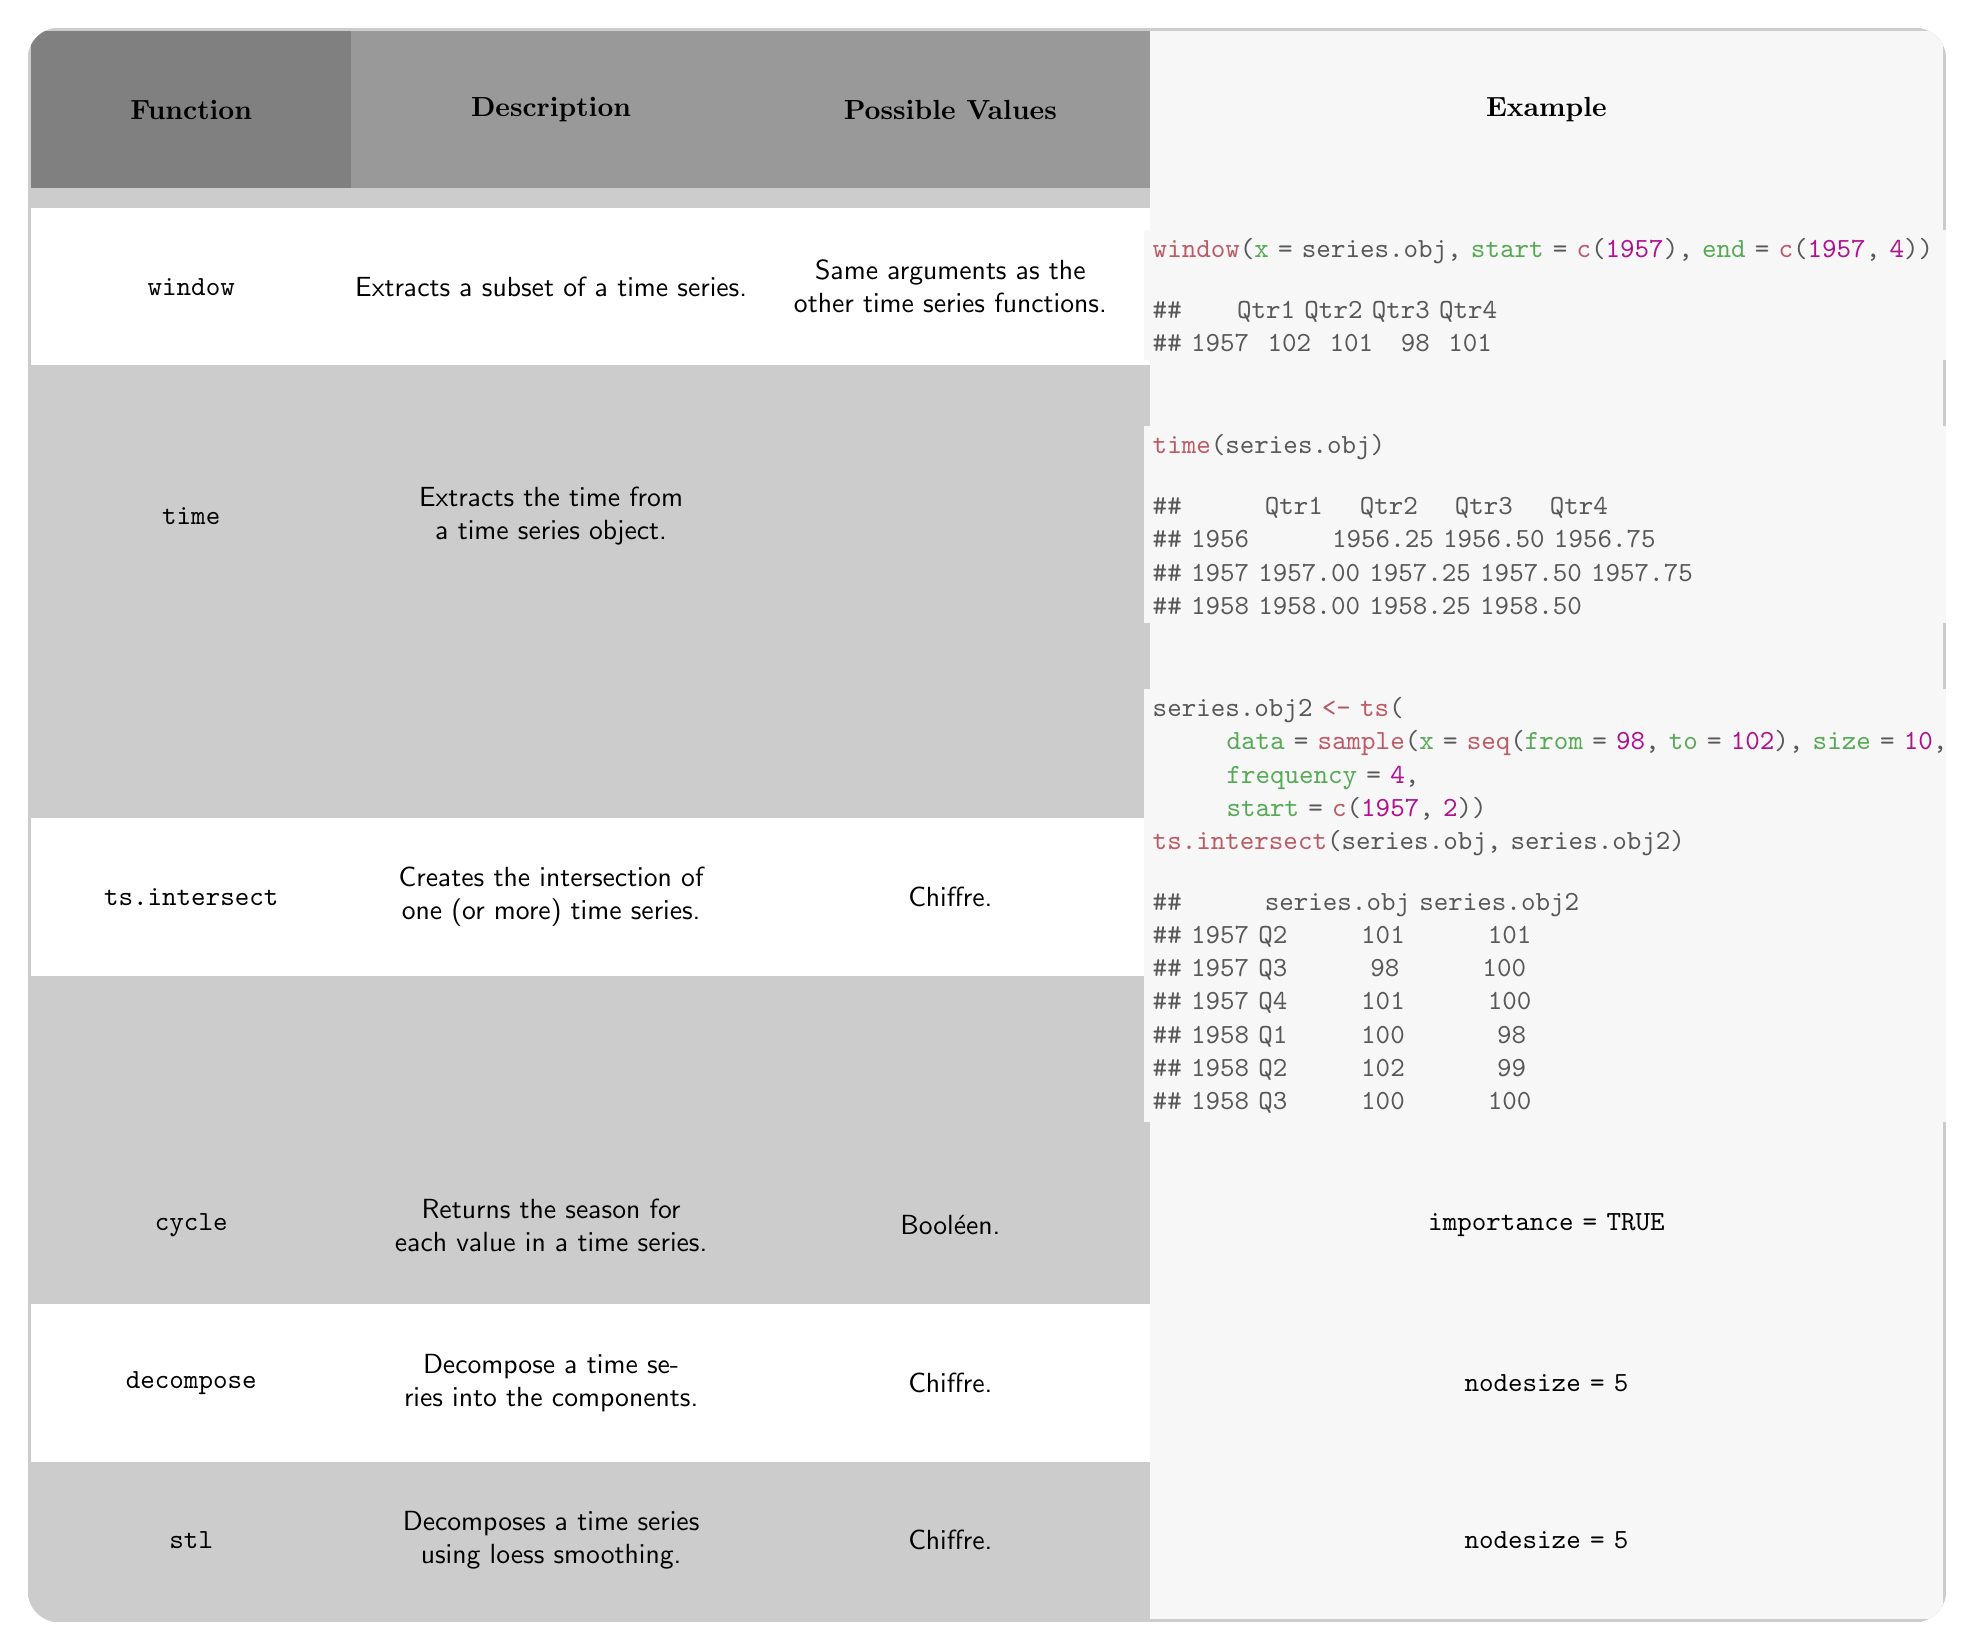
\begin{tikzpicture}
\clip node (m) [
	matrix,
	matrix of nodes,
	fill = black!20, % alternating rows color
	inner sep = 1pt, % width of exterior line
	nodes in empty cells,
	nodes = {
		minimum height = 2cm,
		minimum width = 2.6cm,
		anchor = center,
		outer sep = 0,
		font = \sffamily
	},
	row 1/.style = {
		nodes = {
			text = black,
			font = \bfseries
		}
	},
	column 1/.style = {
		text width = 4cm, 
		align = center,
		nodes = {
			font = \bfseries
		},
		every even row/.style = {
			nodes = {
				fill = white
			}
		}
	},
	column 2/.style = {
		text width = 5cm,
		align = center,
		every even row/.style = {nodes = {fill = white}},
	},
	column 3/.style = {
		text width = 5cm,
		align = center,
		every even row/.style = {nodes = {fill = white}},
	},
	column 4/.style = {
		text width = 10cm,
		align = center,
		nodes = {fill = rstudioblue}
	},
	row 1 column 1/.style = {nodes = {fill = gray}},
	prefix after command = {
		[rounded corners = 4mm] (m.north east) rectangle (m.south west)
	},
	row 1 column 2/.style = {nodes = {fill = gray!80!white}},
	prefix after command = {
		[rounded corners = 4mm] (m.north east) rectangle (m.south west)
	},
	row 1 column 3/.style = {nodes = {fill = gray!80!white}},
	prefix after command = {
		[rounded corners = 4mm] (m.north east) rectangle (m.south west)
	}
] {
	\textbf{Function}	&	\textbf{Description}	&	\textbf{Possible Values}	&	\textbf{Example} \\
	\texttt{window}	&	Extracts a subset of a time series.	&	Same arguments as the other time series functions.  	&	
\begin{knitrout}
\definecolor{shadecolor}{rgb}{0.969, 0.969, 0.969}\color{fgcolor}\begin{kframe}
\begin{alltt}
\hlkwd{window}\hlstd{(}\hlkwc{x} \hlstd{= series.obj,} \hlkwc{start} \hlstd{=} \hlkwd{c}\hlstd{(}\hlnum{1957}\hlstd{),} \hlkwc{end} \hlstd{=} \hlkwd{c}\hlstd{(}\hlnum{1957}\hlstd{,} \hlnum{4}\hlstd{))}
\end{alltt}
\begin{verbatim}
##      Qtr1 Qtr2 Qtr3 Qtr4
## 1957  102  101   98  101
\end{verbatim}
\end{kframe}
\end{knitrout}
	\\
	\texttt{time}		&	Extracts the time from a time series object.	&	 	&	
\begin{knitrout}
\definecolor{shadecolor}{rgb}{0.969, 0.969, 0.969}\color{fgcolor}\begin{kframe}
\begin{alltt}
\hlkwd{time}\hlstd{(series.obj)}
\end{alltt}
\begin{verbatim}
##         Qtr1    Qtr2    Qtr3    Qtr4
## 1956         1956.25 1956.50 1956.75
## 1957 1957.00 1957.25 1957.50 1957.75
## 1958 1958.00 1958.25 1958.50
\end{verbatim}
\end{kframe}
\end{knitrout}
	\\
	\texttt{ts.intersect}	&	Creates the intersection of one (or more) time series. 	&	 Chiffre.	&	
\begin{knitrout}
\definecolor{shadecolor}{rgb}{0.969, 0.969, 0.969}\color{fgcolor}\begin{kframe}
\begin{alltt}
\hlstd{series.obj2} \hlkwb{<-} \hlkwd{ts}\hlstd{(}
        \hlkwc{data} \hlstd{=} \hlkwd{sample}\hlstd{(}\hlkwc{x} \hlstd{=} \hlkwd{seq}\hlstd{(}\hlkwc{from} \hlstd{=} \hlnum{98}\hlstd{,} \hlkwc{to} \hlstd{=} \hlnum{102}\hlstd{),} \hlkwc{size} \hlstd{=} \hlnum{10}\hlstd{,} \hlkwc{replace} \hlstd{= T),}
        \hlkwc{frequency} \hlstd{=} \hlnum{4}\hlstd{,}
        \hlkwc{start} \hlstd{=} \hlkwd{c}\hlstd{(}\hlnum{1957}\hlstd{,} \hlnum{2}\hlstd{))}
\hlkwd{ts.intersect}\hlstd{(series.obj, series.obj2)}
\end{alltt}
\begin{verbatim}
##         series.obj series.obj2
## 1957 Q2        101         101
## 1957 Q3         98         100
## 1957 Q4        101         100
## 1958 Q1        100          98
## 1958 Q2        102          99
## 1958 Q3        100         100
\end{verbatim}
\end{kframe}
\end{knitrout}
	\\
	\texttt{cycle}	&	Returns the season for each value in a time series.	&	Booléen. 	&	\texttt{importance = TRUE} 	\\
	\texttt{decompose}	&	Decompose a time series into the components.	&	 Chiffre.	&	\texttt{nodesize = 5}	\\
	\texttt{stl}	&	Decomposes a time series using loess smoothing.	&	 Chiffre.	&	\texttt{nodesize = 5}	\\
};
\end{tikzpicture}


\end{document}
